% Session 8 -- the Kondo lattice band structure: a flat f level anti-crossing a conduction
% Placement: sec. "Electronic structure of the Kondo lattice: the Kondo insulator", after
% the anti-crossing paragraph.
% Rendered by figures/blender/s08f06_kondo_bands.py, labels in figures/overlays/s08f06_kondo_bands.tex.
\begin{aqmfigure}{fig:s08:kondobands}{Why a lattice of local moments is an insulator, drawn from
(8.21) per spin in one dimension. (a) With the Kondo coupling switched off, (8.21) is a dispersive
conduction band $\varepsilon_{\mathbf k}$ together with a completely flat band of $f$ levels, the
red line. This band is flat because the auxiliary fermions have no hopping of their own, and the two
bands cross at the Fermi level, which gives a metal. (b) A finite hybridization $\gamma_K$ removes
the crossing. The bands repel each other, the states close to the crossing become mixtures of
conduction electron and local moment, and a gap opens exactly where the crossing was. With one $f$
fermion per site from the constraint (8.11) and a half-filled conduction band, the lower hybridized
band is exactly full. So the Fermi level is inside the gap, and the metal has become a \textbf{Kondo
insulator}. The gap grows with $\gamma_K$, and so with the Kondo coupling $J_K$, and the nearly flat
band edges that remain are the reason why the remaining quasiparticles are heavy.}
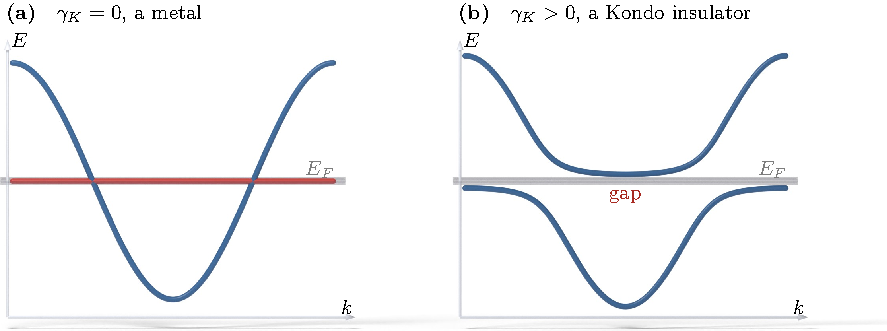
\includegraphics{figures/pdf/s08f06_kondo_bands.pdf}
\end{aqmfigure}
